\documentclass{article}

% if you need to pass options to natbib, use, e.g.:
% \PassOptionsToPackage{numbers, compress}{natbib}
% before loading nips_2016
%
% to avoid loading the natbib package, add option nonatbib:
% \usepackage[nonatbib]{nips_2016}

\usepackage[final]{nips_2016} % produce camera-ready copy
% to compile a camera-ready version, add the [final] option, e.g.:
% \usepackage[final]{nips_2016}

\usepackage[utf8]{inputenc} % allow utf-8 input
\usepackage[T1]{fontenc}    % use 8-bit T1 fonts
\usepackage{hyperref}       % hyperlinks
\usepackage{url}            % simple URL typesetting
\usepackage{booktabs}       % professional-quality tables
\usepackage{amsfonts}       % blackboard math symbols
\usepackage{nicefrac}       % compact symbols for 1/2, etc.
\usepackage{microtype}      % microtypography
\usepackage{blindtext}
% Add graphicx package with pdf flag (must use pdflatex)
\usepackage[pdftex]{graphicx}  
\usepackage{cleveref}
\usepackage{multirow}
\usepackage{graphicx}
\usepackage{subfigure}
\usepackage{appendix}

% Strut macros for skipping spaces above and below text in tables. 
\def\abovestrut#1{\rule[0in]{0in}{#1}\ignorespaces}
\def\belowstrut#1{\rule[-#1]{0in}{#1}\ignorespaces}
\def\abovespace{\abovestrut{0.20in}}
\def\aroundspace{\abovestrut{0.20in}\belowstrut{0.10in}}
\def\belowspace{\belowstrut{0.10in}}

\title{Marketing: Predicting Customer Churn}

% The \author macro works with any number of authors. There are two
% commands used to separate the names and addresses of multiple
% authors: \And and \AND.
%
% Using \And between authors leaves it to LaTeX to determine where to
% break the lines. Using \AND forces a line break at that point. So,
% if LaTeX puts 3 of 4 authors names on the first line, and the last
% on the second line, try using \AND instead of \And before the third
% author name.

\author{
%   Jake Sommers\\
  S1890666\\
%   \texttt{s1890666@ed.ac.uk} \\
  %% examples of more authors
  \And
%   Hao Wang\\
  S1802373\\
%   \texttt{s1802373@ed.ac.uk} \\
 \And
%   Zili Jiang\\
  S1809576\\
%   \texttt{s1809576@ed.ac.uk} \\
 \And
%   Julia Dixon\\
  S1887468\\
%   \texttt{s1887468@ed.ac.uk}\\
}

\begin{document}

\maketitle

\begin{abstract}
 
This project, derived from the KDD Cup 2009 competition, focuses on predicting an element of customer behaviour, customer churn, with preprocessing and classification on the provided anonymised data set.
We adopted exploratory data analysis and explored the feature of the data set, and introduced several simple classifiers and ensemble methods, including Naive Bayes, Logistic Regression, Decision Tree, Bagging, Boosting and Voting classifiers.
This project compared their performance and discussed the potential reasons for the achieved outcome.
\end{abstract}

\section{Introduction}
\subsection{Motivation}
The data set that forms the basis for this assignment was originally prepared for the KDD Cup Challenge 2009.
The data was provided by the French Telecomms company Orange and the task represented a real-life business challenge: creating an effective \emph{Customer Relationship Management} (CRM) model.

CRM is a strategic approach to managing company's interaction with current and future customers with the purpose of driving business growth through improved customer relationship.
The concept of CRM emerged at the end of the 20th century and since then multiple models have been adopted by the business community.
The key aspect of this approach is the development of a customer-centric business culture, which necessitates an in-depth understanding of customer profiles, needs and behaviours \cite{buttle2009customer}.

The complexity of the input space makes modelling such understanding a challenging multi-dimensional task.
The objective of the 2009 KDD Cup competition was to predict three specific aspects of customer behaviour: the propensity of customers to switch the telecomms provider due to the loss of interest in the current service (customer churn); the tendency to sign up for a new product or service (appetency); and the inclination to upgrade or purchase add-ons (upselling) \cite{guyon2009analysis}.

\subsection{Background and Previous Work}

The KDD Challenge is an annual competition that focuses on data mining/machine learning tasks.
In 2009, an offer of a lucrative prize attracted a total of 450 competition entrants, all aiming to achieve better prediction results on the three target variables (\emph{customer churn}, \emph{appetency} and \emph{upselling}) compared to the classification algorithm developed by Orange in-house.
\cite{guyon2009analysis} offered a comprehensive summary of the top successful approaches; and the Cup organisers made the reports authored by the individual teams available for public use. 

The analysis of the literature mentioned above highlighted the key themes about the task (heterogeneous sparse data, large number of training examples, unbalanced class distribution etc) as well as the best practice in achieving a favourable task outcome (e.g.\ utilising ensemble learning methods).
This information inspired the authors of this report to adapt the techniques described as best practice to our project.

\subsection{Project Scoping}

The KDD challenge organisers provided two distinct data sets: a large data set consisting of 15,000 features and a downsized version of the same data set consisting of 230 features.
Both data sets offered a large volume of training examples - 50,000, and a separate test set. 

While the teams on the leader board of the KDD challenge focused their modelling efforts primarily on the large data set, this assignment will concentrate on the exploration of the smaller data set version with the purpose of predicting a single aspect of customer behaviour, the choice of which will be made following the data exploration.
The authoring team considers the selected approach appropriate in the context of the ten credit Data Mining and Exploration module because it will allow the application of a variety of data exploration and modelling techniques without requiring extensive computational power.

The goal of the assignment is to apply best practice techniques to pre-process the data set in such a way that it could be consumed by the selected training model and produce a reasonable level of performance for predicting the target variable.
While the results achieved by the KDD Cup performers will serve as a useful benchmark for this activity, there is no expectation that this team will match the level of performance of the leader board entries.


\section{Data Preparation and Exploration}
\subsection{Class distribution}
The task in hand represented three distinct binary classification problems. 
Since the team's focus was on solving a single problem, the \emph{exploratory data analysis} (EDA) began with establishing the class distribution for each of the targets: appetency, churn and upselling.
A histogram of class distribution (\Cref{fig:cla_dist}) confirmed a significant bias for negative class in all three target variables. 
%A histogram of class distribution was drawn as shown in \Cref{fig:cla_dist}, which confirmed a material bias for negative class in all three target variables. 

\begin{figure}[htbp]
\vskip 5mm
\begin{center}
\centerline{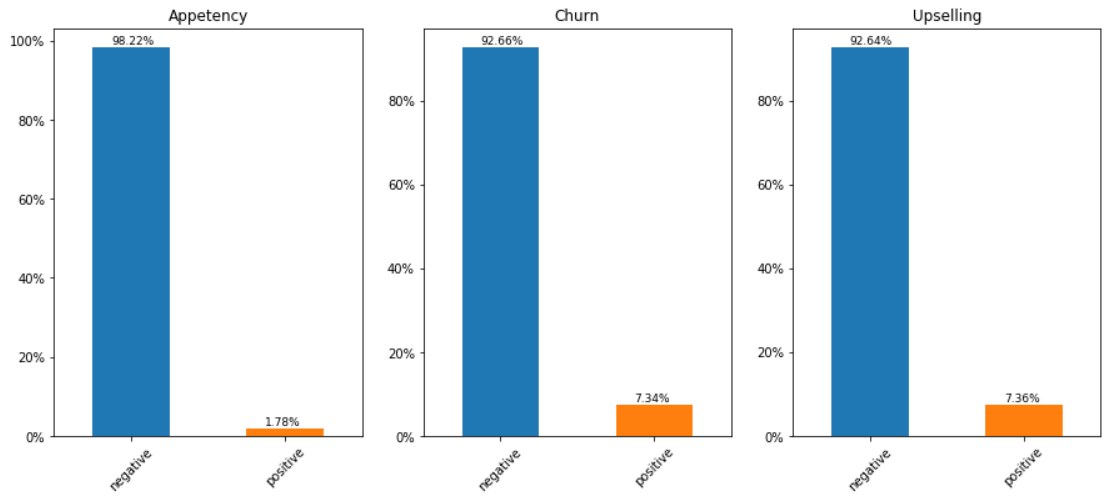
\includegraphics[width=5in]{graph/Class_distribution.PNG}}
\caption{Class distribution in target metrics}
\label{fig:cla_dist}
\end{center}
\vskip -5mm
\end{figure} 

Based on this analysis the team chose customer churn as the aspect of customer behaviour to be modelled.
%behaviour on which the subsequent modelling efforts would be focused.
%focus the subsequent modelling efforts on the customer churn.
The analysis also highlighted that extra care needed to be taken when choosing the prediction model(s) and the evaluation mechanism, as both would need to be suitable for solving a binary classification problem with a significant class imbalance. 

\subsection{Feature exploration and cleaning}
Feature exploration formed the second step of the EDA.
The initial examination of the training data set established that it consisted of 230 features and 50,000 records.
%(190 numeric consisting of 189 float and 1 integer, as well as 40 categorical) and 50,000 records.
The raw data had been fully anonymised by the organisers since it contained information about private customers.
All variable names followed a naming convention of `Var\textit{n}' (where \textit{n} was the index of the column) and all categorical values had been converted into random strings.
This level of data anonymising, although necessary from a privacy perspective, limited the team's understanding of the domain and the ability to apply judgment to identify outliers, among other intuitive decisions.
%Because the data contains information about private customers, we also confirmed that the data had been completely anonymised; in particular, all variable names have been relabelled in to the form `Var\textit{n}' (where \textit{n} is the index of the column) and all categorical values have been converted into random strings.
%As a result, all of the further exploration was based on purely statistical analysis of the features.
%It also meant that we could not use judgment calls when it came to identifying and removing outliers. 
The preliminary exploration had also highlighted a high volume of missing data: almost 70\% of all data were missing.
18 features were removed due to containing no data at all; the remaining feature set was checked for duplicate features but none were present.
Following the first cleaning step, the data set was reduced to 212 features (173 with continuous numeric values and 39 categorical features).

The team intended to backfill the missing numeric values with feature means, however a decision had to be taken on whether to remove a subset of the features with low value coverage or, alternatively, expand the feature set to preserve the information about the missing data by creating new features indicating the presence/absence of data in the original features.
To establish the suitable way forward the team visualised the distribution of features based on the percentage of valid data, presented in \Cref{fig:fea_dist}.
This analysis highlighted that 66 features (circa 31\% of the cleaned feature set) had value coverage in excess of 80\%, whereas 136 features (circa 64\% of the feature set) had value coverage below 10\%.
Removing sparsely populated features would have resulted in a loss of nearly two thirds of the feature set, which the team considered too risky from an information loss perspective.
%which the team did not consider a viable option.
%Furthermore, analysis of the methods used during the KDD competition indicated that PCA had little effect on the quality of the final model \cite{guyon2009analysis}, so the team decided to focus on more traditional dimensionality reduction techniques.

Following this assessment the data set was segregated by data type.
Missing values for  real-valued numeric features were imputed with feature means, and the feature set was expanded by binary encoded features indicating imputed vs originally present values.
Subsequently, a correlation assessment of the numeric features was made, as shown in \Cref{fig:feat_heat}, and features with correlation in excess of 80\% were removed, reducing the numeric feature set by 48 features.
The corresponding encoded features were also removed.
%The team did not consider PCA as an alternative dimensionality reduction method based on the findings documented in the KDD competition analysis \cite{guyon2009analysis}, which suggested that PCA did not prove beneficial for this task.

\begin{figure}[htbp]
\centering

\subfigure[Feature distribution by percentage of valid data]{
\begin{minipage}[t]{0.5\linewidth}
\centering
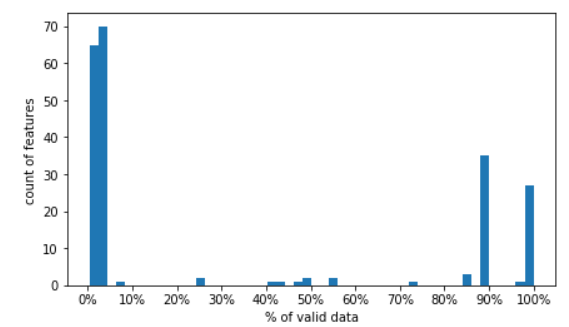
\includegraphics[width=2.5in]{graph/Feature_distribution.PNG}
\label{fig:fea_dist}
\end{minipage}%
}%
\subfigure[Feature correlation heatmap]{
\begin{minipage}[t]{0.5\linewidth}
\centering
\includegraphics[width=2.5in]{graph/Feature_correlation.PNG}
\label{fig:feat_heat}
\end{minipage}%
}%

\centering
\label{fig:ROC}
\caption{Feature visualisations}
\end{figure}

Further exploration was then carried out for the categorical features.
First, the top ten counts for each category for each feature was printed for every categorical feature, which was then visualised using a bar plot that counted for each value of the feature the number of entries in each class.
Due to the extreme class imbalance, it was difficult to determine whether certain features would be a good way to distinguish between the classes, as the underlying distribution of feature categories usually consisted of one category value containing the majority of the entries for that feature. \Cref{fig:3_cat} shows the distribution for a small selection of cateogircal variables.
This analysis did reveal that some of the features contained only one category, with a similar distribution of the classes as in the data set as a whole (i.e.\ class distribution remained at around 10\% positive); since these features would not contain any information to distinguish the classes, they were removed (5 features in total). Since we planned to use one-hot encoding in order to fit linear classifiers to the model, a number of preprocesing steps were required for the cateogircal variables.
In many of the categorical variables, we discovered that there were a large number of distinct categories.
These would greatly boost the size of the one-hot encoding, so the first pass of cleaning involved removing any variable for which there were upwards of 500 distinct categories.
Binning proved to be useful for many of the competition entrants \cite{guyon2009analysis}, so we decided to implement it by creating a new category for each categorical variable, 'OTHERS'.
In this category, we included every category which had less than 5\% coverage of the total number of entries.
Another problem with using one-hot encoding was that some categorical variables had a considerable number of missing values; these were replaced with a new category `MISSING' which can easily be transformed using one-hot encoding.
The effects of these cleaning steps on an example variable can be seen in \Cref{fig:cat_transform}.

\begin{figure}[htbp]
\vskip 5mm
\begin{center}
\centerline{\includegraphics[width=5in]{graph/CategoricalDistribution.png}}
\caption{Class Distribution of three categorical features (Var206, Var207 and Var208)}
\label{fig:3_cat}
\end{center}
\vskip -5mm
\end{figure}

\begin{figure}[htbp]
\vskip 5mm
\begin{center}
\centerline{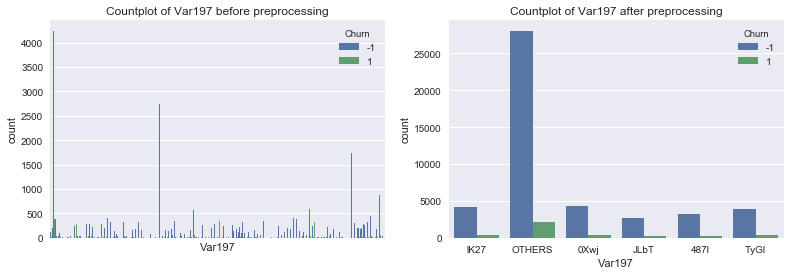
\includegraphics[width=5in]{graph/CountplotDiff.png}}
\caption{Countplots showing changes to Var197 after preprocessing on categorical variables}
\label{fig:cat_transform}
\end{center}
\vskip -5mm
\end{figure}

%Using binning as a further dimensionality reduction method for the categorical variables was considered, but was not implemented due to the anonymous nature of the variables, which meant that there was no way to implement a meaningful binning strategy, especially across the different categorical feature distributions. 

%In order to accommodate for linear classifiers to be able to use the categorical data, we decided to use one-hot encoding, which required further cleaning of the categorical variables.
%The first problem for one-hot encoding was the presence of categories which contained a large number of distinct string values.
%Since this would greatly increase the time taken to train the models, we decided to remove all variables which contained more than 500 categories.
%A second problem was that some categorical variables had a considerable number of missing values; these were replaced with a new category `MISSING' which can easily be transformed using one-hot encoding.
%For the remaining variables, we discovered some categories that only had a small number of occurrences.
%Since they are unlikely to significantly influence the model, these categories were collapsed together into one, denoted by `OTHERS'.
%We collapsed any category which contained less than 5\% of the total number of entries.

%After all data pre-processing steps were completed, the data sets now consisted of 125 numerical and 17??? categorical features (before one-hot encoding was performed) for a total of 142 features, a 38\% reduction in dimensionality. For a train/validation/test split, since we only had access to labels for the training set, we set aside a test set consisting of 10,000 entries at this stage to compare final results.

After above data pre-processing steps were completed, the data sets consisted of 125 numerical and 17/67 categorical features (before/after one-hot encoding was performed).
There were additionally 125 features representing the binary missing value indicators for each numerical column.
Since we were limited in terms of both resources available and training time for our models, we decided to use a traditional dimensionality reduction technique (standard PCA with \emph{sklearn.decomposition.PCA}) as the last pre-processing step for categorical variables.
This was also motivated by our concern that a high number of variables may lead to overfitting because of the sparsity of the data, particularly for logistic regression and decision tree classifiers (although for decision trees this can be counteracted using the max-depth hyper-parameter).
Although many teams taking part in the challenge found little improvement using PCA \cite{guyon2009analysis}, since we undertook our own preprocessing and encoding of the categorical variables that condenses the information, we decided to apply it to the categorical variables only.
The PCA resulted in the top 32 components containing 90\% of the explained variance, which we took as our cut-off point; as a result, the PCA reduced the number of categorical (encoded) features from 67 to 32.
%on top of the preprocessing.

For a train/validation/test split, since we only had access to labels for the training set, we set aside a test set consisting of 10,000 entries (20\%) at this stage to compare the models on.
This test set was generated with $sklearn.model\_selection.train\_test\_split$, with random state parameter set for repeatability.

%\begin{figure}[htbp]
 %\centering 
 %\includegraphics[width=0.9\linewidth,height=10cm,keepaspectratio]{CategoricalDistribution.png}
 %\caption{Class Distribution of three categorical features (Var206, Var207 and Var208)}
 %\label{fig:3_cat}
%\end{figure}


%\subsection{Planned approach}
%The approach to data preparation and exploration will include the following:
%  \begin{itemize}
%  \item  Establish the usefulness of the features by checking that they 1) contain data and 2) are not duplicated. Reduce the initial feature set to useful features only;
%  \item  Identify and segregate numeric and categorical features;
% \item  Establish the share of missing values in the data set and  within each feature type, and decide on the appropriate method for handling them: simple feature mean imputation will be considered as the first option for the numeric features, however if the results prove unsatisfactory a multiple imputation model may be computed. Feature engineering to indicate missing values will also be explored. 
%  \item Determine if any numeric features could be subject to discretization and apply the procedure on them;
%  \item  Establish the distribution of values within the categorical features to decide on the appropriate way of handling them (it is likely that both encoding and binning will be required);
%  \item Establish if feature selection practice could prove useful, and if so, implement appropriate feature selection technique.
%  \item Analyse the distribution of class labels in the training data set.
%\end{itemize}

%Despite the fact that different PCA approaches featured heavily in the DME course content, the team will not consider performing PCA on the data set in question because the approach was highlighted as not useful by multiple contestants.

%\subsection{Findings to date}
%The initial analysis of the data set shows that it consists of 50,000 training examples and 230 features. 18 of the presented features hold no data, which means they offer no value from a modelling perspective and could be removed, thus reducing the useful feature set to 212. The useful feature set is split between 38 (18\%) categorical features and 174 (82\%) numeric features.

\section{Learning methods}
%The explored literature suggests that an ensemble Decision Tree classifier proved the most successful on the large data set, and hence the team will be looking to replicate this practice on the small data set. 
%To avoid overfitting, we will consider appropriate regularisation techniques.  The hyper-parameters such as the regularisation rate or depth of the tree will be selected after applying 5-fold cross-validation.
%Depending on the achieved results, other learning methods may be explored.

In line with the summary of the methods used by successful competitors in the KDD Cup competition \cite{guyon2009analysis}, the team decided to experiment with several different classifiers.
%use a wide range of different classifiers.
The three types of classifier we implemented were Gaussian Naive Bayes (NB), Logistic Regression (LR) and Decision Tree (DT).
Given the sparse nature of the data and the imbalanced class distribution, we chose to use these classifiers with established ensemble methods.
Ensemble methods are algorithms which combine multiple machine learning techniques into a single predictive model to minimise variance (bagging), bias (boosting), or improve predictions (stacking and voting) \cite{ens}.
%we aimed to use these classifiers with pre-existing ensemble methods.
%We also implemented a fourth classifier to act as a baseline for our results: this classifier implemented a binomial distribution using a 10\% positive rate to mimic the distribution of the churn classes.

Three ensemble methods were used with the classifiers: Bagging, Boosting and (soft) Voting Classifier (Voting).
%These methods were applied in an attempt to improve the accuracy of the model. 
%By using sampling methods to (in effect) train on the same training set more than just the once.
%Without these methods, if we train a model then the data set is passed through only once, and we end up with a single model.
When Bagging and Boosting are used with Decision Trees or Logistic Regression, the model is trained iteratively.
In the final classification all of the results provided by each iteration created using the ensemble method are weighted to obtain a more precise result. 
%When we use our final classifier to predict a classification, all of the results provided by each iteration created using the ensemble method are weighted to obtain a more precise result. 

Bagging \cite{bagging} involves picking samples at random from the data set to be used in a training set, and was implemented with both the Decision Tree and Logistic Regression classifiers.
More specifically, given a training data set $D$ with $n$ entries, Bagging generates $m$ new data sets of size $n$ by sampling from $D$ uniformly at random with replacement.
Each of the $m$ created data sets are then used to train the models.
When predicting classification, we obtain $m$ predictions, which are then weighted.

Alternatively, Boosting \cite{buhlmann2010boosting} iterates the regression in the simple classifiers, with different weights being given to samples for each iteration, with the weighting being based on the results of the previous trained iteration - wrong predictions are given heavier weights.
Boosting was applied to the Decision Tree classifier.
In more detail, a data set $D$ of $n$ entries is used to first train a base model, which is used to predict on the data set $D$ - any incorrect predictions are isolated.
These incorrectly predicted entries are used together with $D$ to train a second model, with weights given to the additional data in each step.
This process continues iteratively to train $m$ models, with weights given to predictions based on the accuracy produced on the training data set.

A key difference between these two ensemble methods is that boosting uses all training data, whereas bagging may miss some training entries due to the sampling method used.
Also, since boosting has no effect on linear classifiers (the iterative step would retrain the same weights for a linear model each step), it is not appropriate to use with a Logistic Regression classifier.

In addition, a soft voting method was applied using three types of classifier for comparison.
If we train three models (Decision Tree, Logistic Regression and Random Forest \cite{breiman2001random}) on the training data set, we can use the prediction from each model and take the final prediction to be the most common classification.
A soft Voting classifier additionally applies a probability weight to each of the models for the final prediction.

To simplify notation in graphs and tables, we used the following names for our classifiers: Decision Tree/DT (no ensemble method applied), Random Forest/RF (DT with bagging), AdaBoost (DT with boosting), Logistic Regression/LR (no ensemble method applied), Bagging (Logistic Regression with bagging) and Voting Classifier (Soft Voting classifier).

%In order to tune the hyper-parameters for each model, we used standard 5-fold cross-validation, together with a grid search implemented in \emph{sklearn}.
%Although far from exhaustive due to time conditions, we used a wide range of different hyper-parameter values at this stage: for example, for the Random Forest Classifier we used the values in \Cref{tab:rfc_hyper} to search over: 

%\begin{table}[htbp]
%\vskip 3mm
%\begin{center}
%\begin{small}
%\begin{sc}
%\begin{tabular}{l|l}
%\hline
%\hline
%\abovespace\belowspace
%Hyper-parameter & Values \\
%\hline
%\abovespace
%Number of Estimators & [10, 20, 30, 50, 100, 200] \\
%Max Depth & [5, 8, 10, 15] \\
%\belowspace
%Max Number of Features & [1, 2, 3, 4, 5, 6, 7, 8, 9, 10] \\
%\hline
%\hline
%\end{tabular}
%\end{sc}
%\end{small}
%\newline
%\caption{Hyper-parameter selection grid for Random Forest Classifier.}
%\label{tab:rfc_hyper}
%\end{center}
%\vskip -3mm
%\end{table}

%The best performing hyper-parameters for the Decision Tree classifier with bagging included using 10 estimators and a max depth of 15 for each tree in the Random Forest.
%A regularization rate of 0.1 was used for the Logistic Regression classifier with bagging.
%The AdaBoostClassifier used 10 estimators, a max depth of 8 and a learning rate of 0.5. 

In addition, we decided to train (and test) our models on four variants of our pre-processed dataset, each variant including certain combinations of pre-processed features.
Since we had encountered and understood the mechanics of PCA from the course, we elected to train/test on the data both with and without applying PCA to see if we could explain any difference (although we weren't necessarily expecting any difference due to the results of the competition).
We also trained/tested on the dataset with and without using the added missing value features (annotated as missing matrix) - this was motivated by our ability to easily separate the dataset this way, so we could see directly if this made any difference to each classifier. %This resulted in training and testing the classifiers on four variants of our pre-processed dataset.

\section{Performance Analysis}

%\begin{figure}[htbp]
 %\centering 
% \includegraphics[width=0.9\linewidth]{Feature_correlation.PNG}
 %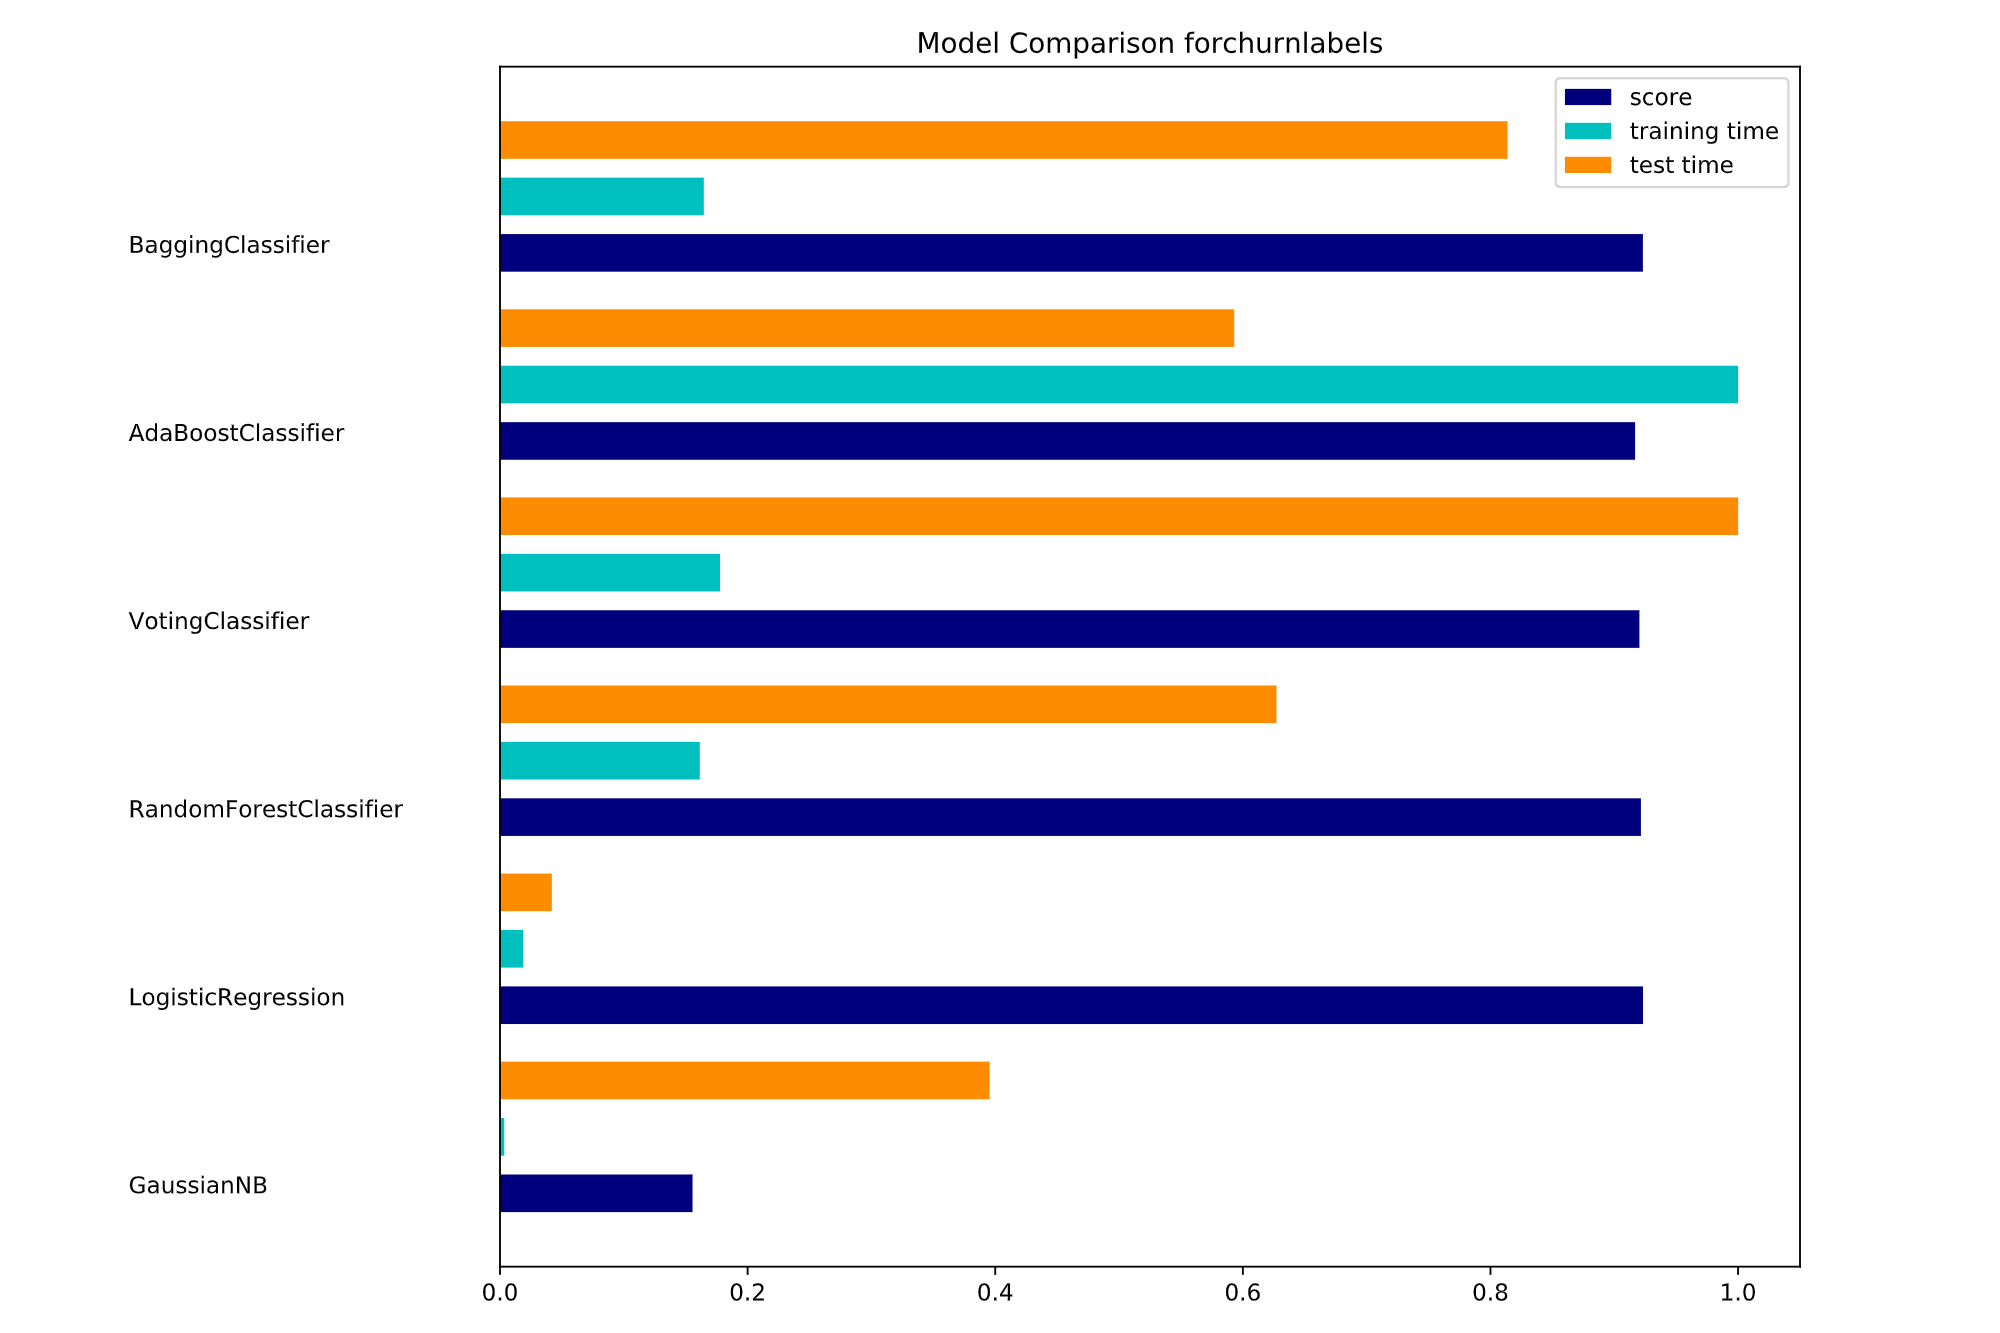
\includegraphics[width=0.9\linewidth,height=10cm,keepaspectratio]{ModelComparisonChurn.png}
 %\caption{Model Performance Comparison}
 %\label{fig:model_com}
%\end{figure}

%\begin{table}[htbp]
%\vskip 3mm
%\begin{center}
%\begin{small}
%\begin{sc}
%\begin{tabular}{c|cccc}
%\hline
%\hline
%\abovespace\belowspace
%Approach & TPR(\%) & FPR(\%) & TNR(\%) & ACC(\%) \\
%\hline
%\abovespace
%NB & 92.97 & 90.89 & 9.11 & 15.55 \\
%LR & 0.13 & 0.01 & 99.99 & 92.32 \\
%DT & 8.46 & 8.48 & 91.52 & 85.14 \\
%RF & 0.39 & 0.22 & 99.78 & 92.15 \\
%Voting & 1.17 & 0.41 & 99.59 & 92.03 \\
%AdaBoost & 1.56 & 0.82 & 99.18 & 91.68 \\
%\belowspace
%Bagging & 0.26 & 0.01 & 99.99 & 92.31 \\
%\hline
%\hline
%\end{tabular}
%\end{sc}
%\end{small}
%\newline
%\caption{TPR, FPR, TNR and ACC for models implemented in our project (churn).}
%\label{tab:prediction_result}
%\end{center}
%\vskip -3mm
%\end{table}

Due to the significant class imbalance present in the data, we have reported not only the accuracy but the precision, true positive (TP) and false positive (FP) rates for each classifier across the four dataset variants in \Cref{tab:result_nomiss} and \Cref{tab:result_miss}.
As shown in \Cref{fig:ROC}, we provided a visualisation of the ROC curve for each model and labelled the area under each curve, as this is not only a widely used statistic for model comparison, but was also used as the method for scoring the models in the original competition \cite{guyon2009analysis}.

% accuracy (ACC), TPR, FPR, precision (P)
\begin{table}[htbp]
%\vskip 3mm
\begin{center}
\begin{small}
\begin{sc}
\begin{tabular}{c|cccc|cccc}
\hline
\hline
\abovespace\belowspace
\multirow{2}*{Approach} & \multicolumn{4}{c|}{No PCA} & \multicolumn{4}{c}{PCA} \\ \cline{2-9}
\abovespace\belowspace
 & ACC(\%) & TPR(\%) & FPR(\%) & P(\%) & ACC(\%) & TPR(\%) & FPR(\%) & P(\%) \\
\hline
\abovespace
NB & 16.55 & 93.10 & 89.82 & 7.94 & 16.43 & 93.36 & 89.97 & 7.95 \\
LR & 92.32 & 0.00 & 0.01 & 0.00 & 92.31 & 0.00 & 0.01 & 0.00 \\
DT & 85.20 & 11.20 & 8.64 & 9.73 & 86.20 & 14.58 & 7.84 & 13.40 \\
RF & 92.32 & 0.00 & 0.00 & - & 92.32 & 0.00 & 0.00 & - \\
Voting & 92.31 & 0.00 & 0.01 & 0.00 & 92.31 & 0.00 & 0.01 & 0.00 \\
AdaBoost & 92.06 & 1.82 & 0.43 & 25.93 & 91.87 & 1.95 & 0.65 & 20.00 \\
\belowspace
Bagging & 92.31 & 0.00 & 0.01 & 0.00 & 92.31 & 0.00 & 0.01 & 0.00 \\
\hline
\hline
\end{tabular}
\end{sc}
\end{small}
\newline
\caption{Result without missing matrix, accuracy (ACC), TPR, FPR, precision (P)}
\label{tab:result_nomiss}
\end{center}
\vskip -3mm
\end{table}

\begin{table}[htbp]
%\vskip 3mm
\begin{center}
\begin{small}
\begin{sc}
\begin{tabular}{c|cccc|cccc}
\hline
\hline
\abovespace\belowspace
\multirow{2}*{Approach} & \multicolumn{4}{c|}{No PCA} & \multicolumn{4}{c}{PCA} \\ \cline{2-9}
\abovespace\belowspace
 & ACC(\%) & TPR(\%) & FPR(\%) & P(\%) & ACC(\%) & TPR(\%) & FPR(\%) & P(\%) \\
\hline
\abovespace
NB & 17.34 & 92.84 & 88.94 & 7.99 & 17.22 & 93.10 & 89.09 & 8.00 \\
LR & 92.31 & 0.00 & 0.01 & 0.00 & 92.31 & 0.00 & 0.01 & 0.00 \\
DT & 85.27 & 12.50 & 8.68 & 10.70 & 85.56 & 14.19 & 8.50 & 12.19 \\
RF & 92.32 & 0.00 & 0.00 & - & 92.32 & 0.00 & 0.00 & - \\
Voting & 92.31 & 0.00 & 0.01 & 0.00 & 92.31 & 0.00 & 0.01 & 0.00 \\
AdaBoost & 92.04 & 2.08 & 0.48 & 26.67 & 91.97 & 1.82 & 0.53 & 22.22 \\
\belowspace
Bagging & 92.31 & 0.00 & 0.01 & 0.00 & 92.32 & 0.00 & 0.00 & - \\
\hline
\hline
\end{tabular}
\end{sc}
\end{small}
\newline
\caption{Result with missing matrix, accuracy (ACC), TPR, FPR, precision (P)}
\label{tab:result_miss}
\end{center}
\vskip -3mm
\end{table}

For our data, with its material class imbalance, a model which only ever predicts a negative class would produce a high accuracy of 92.3\%.
%since the positive class only made up around 10\% of all entries,
Therefore also reporting the precision, true positive and false positive allows us to see how well our models are identifying the positive class entries using various metrics, since we would want a classifier that classifies as many positive instances correctly, without also generating too many false positives.
Therefore we look for a high True Positive rate and precision with as low a False Positive rate as possible.

The investigation into the use of PCA and the missing data indicators showed little change in the results.
In general, we found that the use of PCA caused little or no improvement (and in a few cases, they were slightly worse) to each of the classifiers.
For example, the Decision Tree classifier had a higher accuracy (85.2\% to 86.2\%), True Positive rate (11.2\% to 14.58\%) and precision (9.73\% to 13.4\%) with a lower False Positive rate (8.64\% to 7.84\%) (when not using the missing indicators), with similar small improvements also when using PCA with the missing indicators.
However, many classifiers, including Logistic Regression, Random Forest, Bagging and Voting Classifier saw no change when using PCA.
AdaBoost, interestingly, had a worse performance when using PCA with the missing indicators, although both the TP and FP rate both increased when using PCA without the missing indicators, so in both cases PCA seemed to have a small net negative effect on AdaBoost.
Naive Bayes was the only classifier which showed worse performance in both cases when using PCA.
Additionally, every classifier showed at most a 0.02 in area under the ROC curve improvement when using PCA.
Overall, we conclude that PCA had little effect on the classifiers, with any change dependent on the classifier.

It was a similar outcome when using the missing indicators.
The same classifiers, Logistic Regression, Random Forest, Bagging and Voting Classifier saw no change.
Only small changes were observed for Naive Bayes. Decision Tree and AdaBoost - in each case, there was a trade-off between better and worse rates when using the missing indicators, with only Decision Tree showing an improvement in every metric when not using the missing indicators.

The results for each classifier however showed a much more interesting outcome.
Naive Bayes was unique in that it consistently showed a very low accuracy rate (around 16-17\%) across all datasets - this was due to it classifying too many entries in the positive class.
It tended to capture most of the positive entries (TP rate of 93\%) but also classified around 90\% of the negative class as positive.
Four classifiers (Logistic Regression, Random Forest, Voting Classifier and Bagging) showed the complete opposite problem - they all classified (almost) everything as negative, as can be seen in the 0\% values for the precision, TP and FP rates.
They did report the highest accuracy amongst all classifiers, but this was only due to the class imbalance.
The conclusion for these classifiers was that none of them offered an acceptable level of performance for the overall task - for Naive Bayes, too many false positives would be returned, whereas the others were equivalent to a base classifier that classified everything as negative.

We found that two of the classifiers showed a small amount of promise - Decision Tree and AdaBoost.
The Decision Tree classifier generated the highest TP rate of 11-14\%, meaning this was the classifier that was finding the most correctly positive entries (outside the extreme result of Naive Bayes).
However, this result came with a trade-off: The FP rate of 8-9\%.
Due to the class imbalance, this meant that the precision is only around 10-13\%.
For the task, this meant that the Decision Tree identified correctly a decent number of positive entries, but also falsely identified many more.
For AdaBoost, the results showed that it was more reluctant to classify instances as positive, since it had a much lower TP rate (around 2\%) but also a much lower FP rate (around 0.5\%) than the Decision Tree classifier.
This could also be seen in the higher precision rate that exceeded 20\%.
The AdaBoost classifier was therefore more sure when it made a positive decision; however, the TP rate was so much lower that it didn't correctly classify many positive entries at all.
Finally, across all four different dataset combinations, the best performing Decision Tree was on the PCA without missing indicators data, whereas AdaBoost performed best on the no-PCA with missing indicators data.
We found that, for the case of customer churn, the area under the ROC was a poor measure as to the usefulness of the model - the models exhibiting an expected behaviour from a business perspective had consistently scored a lower area under the curve than the classifiers predicting only the negative results.
%although their behaviours were closest to what we would want, they consistently scored a lower area than most of the other classifiers excluding Naive Bayes (especially since some of those predicted everything negative).
%From the results, we can see that Logistic Regression and Bagging Logistic Regression achieve the highest accuracy of 92.3\%, with Random Forest and the Voting classifier also achieving over 92\%.
%However, the AdaBoostClassifier, whilst reaching only 91.7\% accuracy, has the highest true positive rate of 1.56\% of these five classifiers, and so would provide the most useful for the task at hand.
%Notably across all classifiers, the true positive rate is very low, with only the Decision Tree and Naive Bayes correctly predicting more than 2\% of the positive class, although in both cases this comes with a trade-off in terms of overpredicting the positive class, as can be seen by their relatively higher false positive rates. Naive Bayes, in particular, has a True Negative Rate of 9.11\%, meaning that this classifier  

Some of the results could be explained using the underlying mechanics of each of the models.
Naive Bayes, for example, could show a strong bias towards positive class prediction because there was a lack of conditional independence between features (perhaps evidenced by the high correlation between numerical variables).
The behaviour of Logistic Regression and its Bagging counterpart could be explained by the major class imbalance and the setting of the decision boundary using the logistic function - we set the decision boundary at 0.5, although a lower value may have been more appropriate in this case.
Because of the high bias and low variance present in a normal Random Forest classifier, combined with our pre-processing steps, the Random Forest classified everything as negative.
The AdaBoostClassifier put emphasis on the positive class labels during its iteration process, so it had a higher true positive rate than the Random Forest model, but it sacrificed for lower accuracy as it produced more false positives.
The Voting Classifier, because it contained two all-negative classifiers, acted the same as an all-negative classifier due to the voting mechanism.

% \begin{figure}[htbp]
%  \centering 
% % \includegraphics[width=0.9\linewidth]{Feature_correlation.PNG}
%  \includegraphics[width=0.9\linewidth,height=10cm,keepaspectratio]{ROCChurn.png}
%  \caption{ROC curve for churn task}
%  \label{fig:roc}
% \end{figure}

\begin{figure}[htbp]
\centering

\subfigure[missing matrix removed and no PCA]{
\begin{minipage}[t]{0.5\linewidth}
\centering
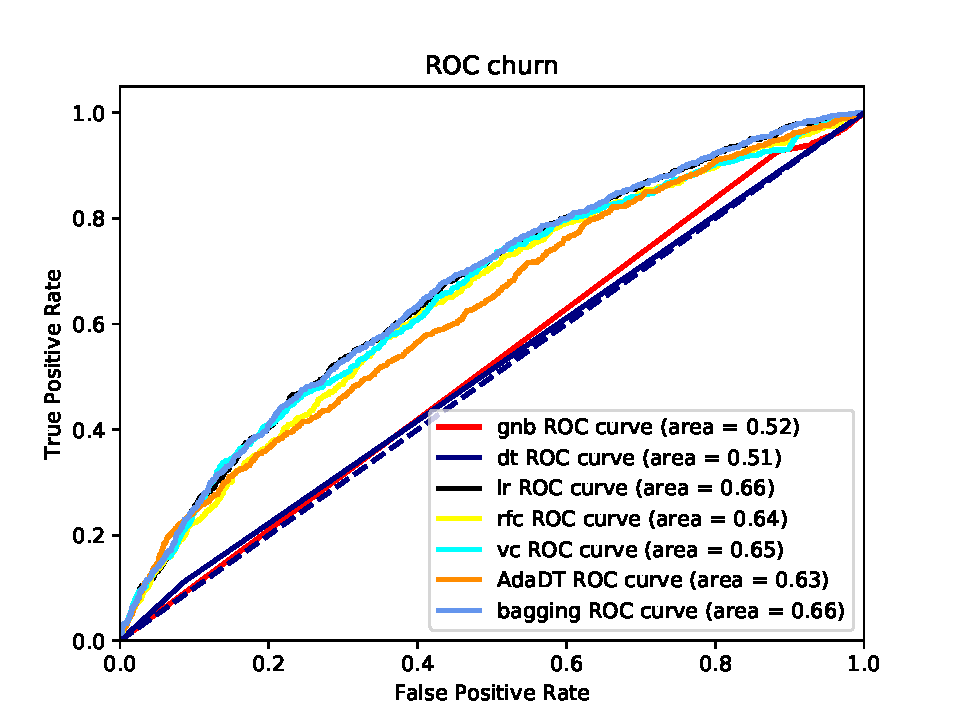
\includegraphics[width=2.5in]{graph/ROC_n_noPCA.pdf}
\label{fig:ROC_n_noPCA}
\end{minipage}%
}%
\subfigure[missing matrix removed but use PCA]{
\begin{minipage}[t]{0.5\linewidth}
\centering
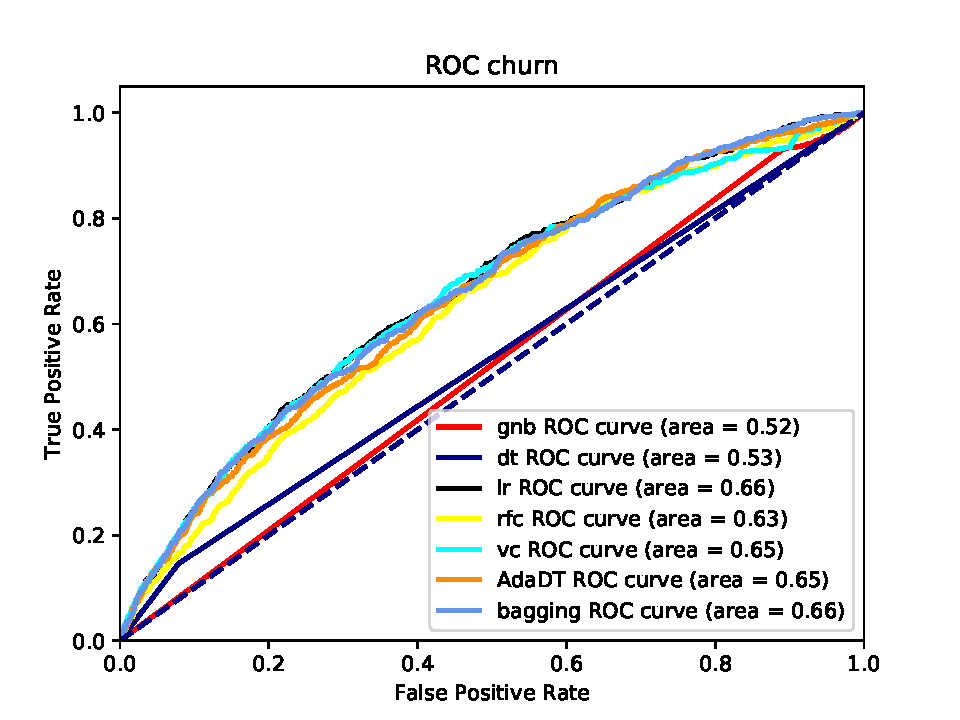
\includegraphics[width=2.5in]{graph/ROC_n_PCA.pdf}
\label{fig:ROC_n_PCA}
\end{minipage}%
}%

\subfigure[missing matrix included but no PCA]{
\begin{minipage}[t]{0.5\linewidth}
\centering
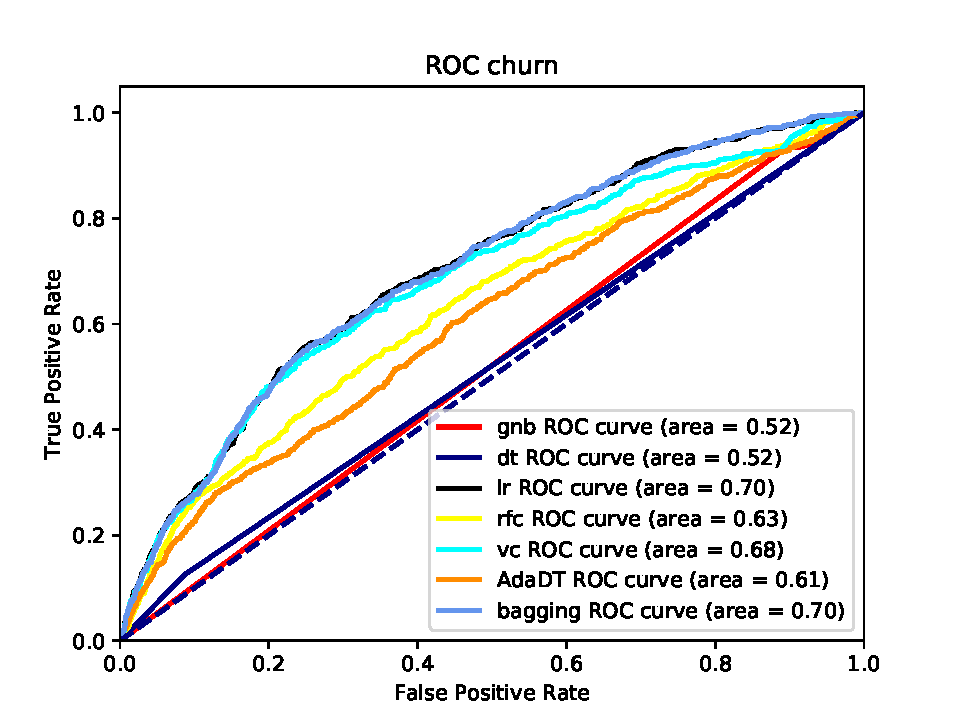
\includegraphics[width=2.5in]{graph/ROC_y_noPCA.pdf}
\label{fig:ROC_y_noPCA}
\end{minipage}
}%
\subfigure[missing matrix included and use PCA]{
\begin{minipage}[t]{0.5\linewidth}
\centering
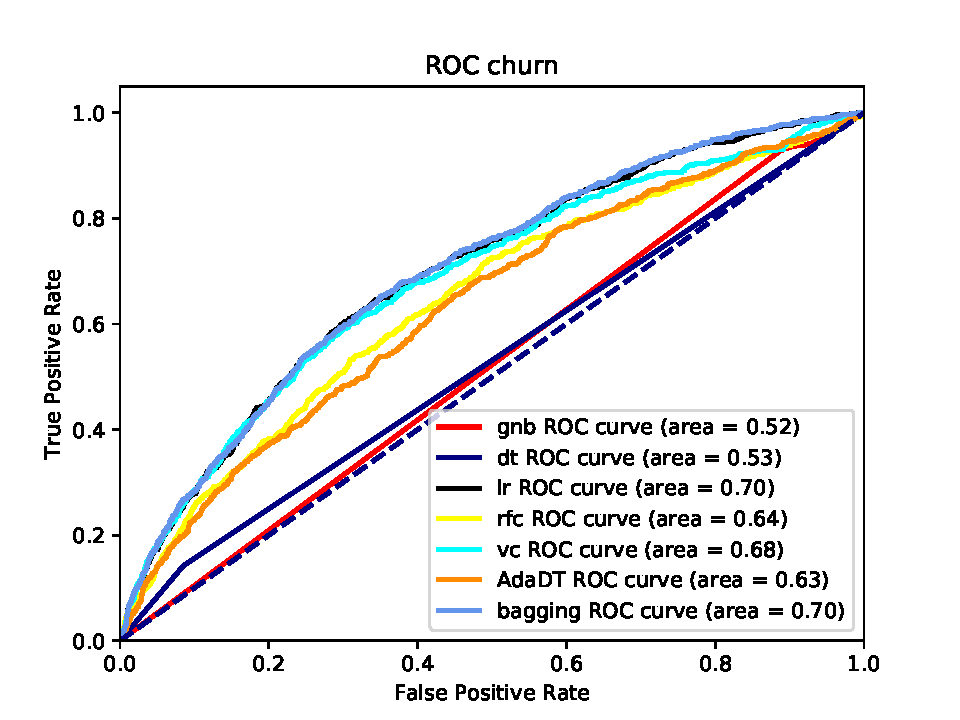
\includegraphics[width=2.5in]{graph/ROC_y_PCA.pdf}
\label{fig:ROC_y_PCA}
\end{minipage}
}%

\centering
\label{fig:ROC}
\caption{ROC curve}
\end{figure}

\section{Conclusion}

The results of our experiments show than none of the classifiers were well suited to the given task with the chosen pre-processing methods, in particular Logistic Regression and others ended up classifying everything as negative.
We conclude that this outcome could be attributed to two main factors:
%there were two major factors to cause this: 
first, our pre-processing techniques were not as powerful at maximising the information as we would have liked, 
%(we focused on traditional methods that we easily understood), 
either because we lost too much information or because the pre-processed data still contained too much noise.
Secondly, the small dataset did not contain the combination of features valuable for more accurate predictions (we worked with 230 features vs. 15,000 in the large dataset).
%causing our results to be below those reported as part of the competition. 
Notably, the leading competition entrants came to the same conclusion and discarded the small dataset in favour of the large one.\cite{guyon2009analysis}

However, two of the classifiers showed promise, namely Decision Tree and AdaBoost, as both had seemingly extracted some useful information from the data in order to classify some positive churn customers.
In our best case scenario, Decision Tree correctly predicted around 15\% of the customers who could switch to a different provider, giving the company an opportunity to influence these customers through incentives.
The downside was that they would also try to incentivise a large number of customers who had no intention to switch.
AdaBoost carried a smaller rate of customers falsely classified as likely to switch, but also only predicted at most 2\% of the total customers who were actually likely to switch.
Some further cost-benefit analysis would be required to determine which of these two models was the most useful for the problem task, which was outside of our scope.
With further time, we would perhaps focused on more powerful pre-processing methods, for example down sampling, as evidenced in \cite{domingos1999metacost}, in order to reduce the severe class imbalance.

%(Future Work by the end?)
%Down-sampling on negative population %\cite{domingos1999metacost,van2007experimental,xie2009combination}.

%1 Data distribution
%After the data preprocessing, we get 125 numeric variables and 17 categorical variables.

%2 Feature engineering
%As the categorical variables are not able to apply to most of the classifier models. We use one-hot encoding to represent the category features. For dimension reduction purpose, we apply PCA. According to the graph shown below, the first 32 components will contain most of the information of the features, so we get 32 features at last to form our dataset.

%3 Models and results
%We will use binominal distribution of 10% successful rate to sample the results for the base line. There are many models for the classification problems. Our main target is to train different models and compare their effects for finding the most powerful models for the problems. The basic classifier models are Na ̈ıve Bayesian, logistic regression and decision tree. They are weak classifiers and we will use the ensemble methods to increase their power of prediction. The two main popular methods are bagging and boosting. Bagging means that we will pick samples from the dataset randomly, so some samples in the dataset may never be trained in the model. We apply bagging to decision tree (random forest), and logistic regression. After running 5-fold cross-validation, we use the 10 estimators and 15 max depth for the random forest and 0.1 regularization rate for the logistic regression to pretend over-fitting. Boosting means that we iterate the regression in the weak classifiers, each iteration will give different weights to the samples. All the samples in the dataset will be used to train the model, but their weights will be updated each time according to the last training results. The wrong predictions will be given heavier weights. And we will combine all the results produced from the iteration. The more precise one will be given more attention. The boosting method will be applied to the decision tree method (AdaBoostClassifier), the hyper-parameters are 10 estimators, 8 max depth and 0.5 learning rate. At last, we will use soft voting method to the Gaussian Na ̈ıve Bayesian, logistic regression and random forest. From the results, we can observe that the accuracy of the logistic regression and bagging logistic regression is highest (both of them are 92.3%). The random forest gets the second highest accuracy (92.15%), the voting classifier has the third highest accuracy (92.03%), but the AdaBoost Classifier has the highest hit rate of “yes” (1.56%).

%\section{Something to add}
%\subsection{Preprocessing of the Category Variables}
%We use the following strategy to preprocess the categorical variables.:
%First, we count how many categories in each categorical variable, we notice that some categorical variables have a lot of categories. As too many categories will make no effort when training the classifier models, we delete the categorical variables which contain more than 500 categories. 

%Second, we replace the missing category as category ‘Missing’. 

%Third, we observe that some categorical variables contain categories which appear just a few times. As our propose is to find the categories which have representative power to identify the samples’ characters, we don’t need the categories which show up less than 5\% of the total samples’ number. We call this kind of category as ‘collapsed category’, and we will replace them as category ‘OTHERS’. 

%At last, we delete the categorical variables which contain only one category except for ‘Missing’ and ‘OTHERS’. 

%\subsection{Split the dataset into Train and Test}
%As we can’t find the test dataset of ‘Y’ in website. We only be able to split the training dataset which contains 50,000 samples into train and test datasets. The test dataset have 10,000 samples, the train dataset includes 40,000 samples.

%\subsection{One-hot encoding}
%After preprocessing, we have 163 numeric variables and 17 categorical variables containing 29 categories. After one-hot encoding, we have total 192 variables. The one-hot encoding processing is done by function in ‘pandas’ package.

%\subsection{PCA}
%We use standard PCA which is a function included in the ‘sklearn.decomposition’ package. As we finally get 192 variables, the large number of variables will increase the depth of the decision tree. When we train the decision tree, we set the hyper-parameter ‘max-depth’ to prevent over-fitting. If we don’t use PCA to reduce the dimensions, many data will be abundant when training the decision tree. When training the logistic regression, 192 variables easily lead to over-fitting as well, so we decide to use standard PCA here. The competitive reports find the standard PCA useless as their data preprocessing of categorical variables are different from us.

%\subsection{The Bagging and Boosting}
%The bagging and boosting are used to improve accuracy of the classifier models. If we use the decision tree or logistic regression to train the model, the dataset will be trained only once, and we get only one model to do the prediction. If we use bagging or boosting, we train the decision tree or logistic regression iteratively. When we need to predict, we weight all the results produced by the iterative models and get a more precise result. So I will say that it is not only suitable for our dataset, it is a common method. 
%\begin{itemize}
%    \item Bagging:
%    Assume that we have one dataset D of size n, we generate m new datasets of size n by sampling from dataset D uniformly and with replacement. Then we use the m new datasets to train our models, and we get m predictions. At last, we weight the m predictions to get a final prediction.
%    \item Boosting:
%    Assume that we have one dataset D of size n. And the weak classifier we use is decision tree. First, we use the dataset D of size n to train the first decision tree. Then we identify the wrong predictions of data i. We use the dataset D of size n with identified data i to train the second decision tree, we give a new weight to the identified data i when training the model, we again identify the wrong predictions of the second decision tree. We repeat the processes and get m decision trees, we give different weights to their predictions according to their accuracies produced by training dataset. 
%    \item VotingClassifier:
%    It is another ensemble method different from bagging and boosting. Assume that we have a dataset D of size n, we use decision tree, logistic regression and random forest to train the dataset D at the same time and make a prediction respectively. Suppose that we get prediction of ‘class 1’ for decision tree and logistic regression and ‘class 2’ for random forest, we will decide the sample to be ‘class 1’ as two classifier models predict it as ‘class 1’. It is called hard voting classifier. If we give different probabilistic weights to the three models, we call it as soft voting classifier. The soft voting classifier in ‘sklearn’ is a black box for the weights. 
%\end{itemize}

%\subsection{The Cross-Validation and Hyper-parameters}
%The cross-validation is a method to tune the hyper-parameters and doesn’t relate to the bagging or boosting. The cross-validation means that we split the training dataset into training and validation datasets. We use the training dataset to train the model and use the validation dataset to tune the hyper-parameters. We can use the first 1/5 portion of the training dataset as validation dataset first time. Then we can use the second 1/5 portion of the training dataset as validation. So we can tune the hyper-parameters five times and use the best one. It is called 5-fold cross-validation.

%\subsection{The name relationship}
%We first try three weak classifiers: decision tree, logistic regression and Naïve Bayes. Then we use bagging to improve two weak classifiers: decision tree (random forest) and logistic regression. Then we use another method (boosting) to improve the decision tree (AdaBoostClassifier), the boosting of logistic regression is not popular. At last, we try the voting classifier, we use three popular classifiers to vote, they are decision tree, logistic regression and random forest. 

%\subsection{The results}
%As the data is imbalanced, we should not only improve the accuracy but also focus on the hitting rate of ‘Yes’ which has low percentage in the dataset. If the model predicts the results all ‘No’, it will have a good accuracy as ‘No’ is a right prediction for most of the samples. Although the hyper-parameters chosen from the cross-validation will produce higher accuracy, the ‘Yes’ hitting rates are low in all models. We decide to use the hyper-parameters tuned by hand. The Naïve Bayes gets the lowest accuracy, as the assumption of Naïve Bayes is conditional independent which is broken apparently. The logistic regression has the highest accuracy but the rate of hitting ‘Yes’ is low. As the data preprocessing, we delete the noise containing in the dataset and leave the most representative variables, the logistic regression is suitable for the dataset, but the turning point or outliers will be easily missed which is an obvious disadvantage of the regression method. So the accuracies of logistic regression and bagging of logistic regression are good, but the hitting rates of ‘Yes’ are low. The AdaBoostClassier will pay more attention to the label of ‘Yes’ when training the dataset during the iteration, so it has the highest rate of hitting ‘Yes’, but accuracy is low. The random forest has a balanced result between accuracy and hitting rate of ‘Yes’. 

%\subsection{Hyper-parameter}
%In this project, we use sklearn.model\_selection.GridSearchCV to select the best hyper-parameter. With this method, we only need to select which hyper-parameters are expected to be selected, and it will search exhaustively over these hyper-parameter settings and return the best combination. For example, for random forest classifier, we choose hyper-parameters from the following set: 'n\_estimators': [10, 20, 30, 50, 100, 200], 'max\_depth': [5, 8, 10, 15], 'max\_features': [1, 2, 3, 4, 5, 6, 7, 8, 9, 10]. The best setting will be returned automatically as “best\_params\_”: {'max_depth': 5, 'max_features': 1, 'n_estimators': 10}



% \newpage
%                Now build the reference list
\bibliographystyle{unsrt}   % The reference style
%                This is plain and unsorted, so in the order
%                they appear in the document.


\bibliography{main}       % bib file(s).

\newpage

\appendixtitleon
\appendixtitletocon
\begin{appendices}
% \textbf{At the end of the report, you must include a short description of how each member of the group contributed to the project, which can be on an additional ninth page.}
\section{Contribution}
s1890666 - carried out categorical variable exploration (in Jupyter notebook), compiled information for and wrote Learning Methods, Performance Analysis and Conclusion

S1802373 - compiled all the python code file (*.py); draw the ROC curves; compiled graphs and tables in this report and wrote Abstract

S1809576 - wrote the code of the categorical variable pre-processing and PCA, provided information and wrote Learning Methods, Performance Analysis and Conclusion

S1887468 - performed the initial exploratory data analysis and visualisations (in Jupyter notebook), data clean up and and the pre-processing of the numeric variables.
Prepared the introduction section of the report, contributed to the Data preparation and Conclusion sections.
\end{appendices}

\end{document}
